\begin{block}{Fluent}
  \begin{CPP}
fluent(name, addr, &context, config)
  .table<int, int>("t", {{"x", "y"}})
  .scratch<int, int>("s", {{"a", "b"}})
  .channel<string, int, int>("c", {{"addr", "u", "v"}})
  .RegisterRules([&](auto& t, auto& s, auto& c) {
    auto rule1 = s <= t.Iterable();
    auto rule2 = t <= c.Iterable() | project<1, 2>();
    return std::make_tuple(rule1, rule2);
  })
  \end{CPP}

  \vspace{1cm}

  \begin{center}
    \ttfamily
    \begin{tabularx}{0.15\textwidth}{|X|X|}
      \hline\rowcolor{red!20}
      \textbf{x} & \textbf{y} \\\hline
      19         & 39 \\\hline
      49         & 1 \\\hline
      9          & 39 \\\hline
    \end{tabularx}
    \hspace{1cm}
    \begin{tabularx}{0.15\textwidth}{|X|X|}
      \hline\rowcolor{green!20}
      \textbf{a} & \textbf{b} \\\hline
      3          & 192 \\\hline
      39         & 191 \\\hline
      29         & 1 \\\hline
    \end{tabularx}
    \hspace{1cm}
    \begin{tabularx}{0.4\textwidth}{|X|l|l|}
      \hline\rowcolor{blue!20}
      \textbf{addr}  & \textbf{u} & \textbf{v} \\\hline
      127.0.0.1:8000 & 19         & 48 \\\hline
      127.0.0.1:8000 & 49         & 5 \\\hline
      127.0.0.1:8000 & 1          & 7 \\\hline
    \end{tabularx}
  \end{center}

  \vspace{1cm}

  \begin{center}
    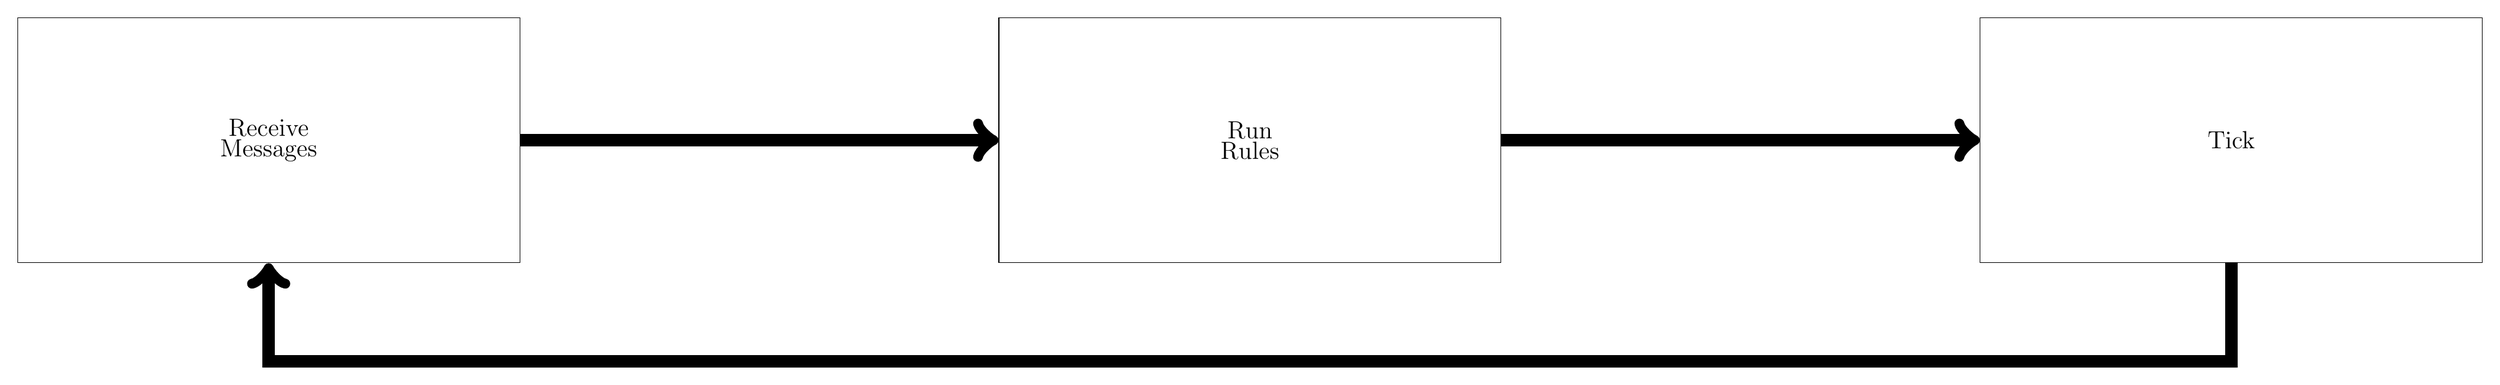
\begin{tikzpicture}
      \tikzstyle{box}=[draw, minimum width=10cm, minimum height=5cm, text
                       width=10cm, align=center]
      \tikzstyle{arrow}=[line width=0.25 cm, ->]
      \node[box] (recv)  at (0, 0)  {\Large Receive\\Messages};
      \node[box] (rules) at (20, 0) {\Large Run\\Rules};
      \node[box] (tick)  at (40, 0) {\Large Tick};
      \draw[arrow] (recv) -- (rules);
      \draw[arrow] (rules) -- (tick);
      \draw[arrow] (tick.south) -- ++(0, -2) -| (recv.south);
    \end{tikzpicture}
  \end{center}
\end{block}
